\begin{itemize}
\item At time 0, normally incident radiation impinges on the left side of a vacuum filled domain
\item Expected result: propagation of a Heaviside wave front in a void to the right. 
\item The \underline{\bf standard Galerkin} FEM scheme produces unphysical oscillations and negativities
\item These are remedied with the \underline{\bf FCT scheme} {\it without}
introducing the amount of diffusion required by the \underline{\bf low-order scheme}. 
\item The high-order scheme based on entropy viscosity {\it without FCT} mitigates the formation of
oscillations but ultimately \underline{still produces some negativities}
\end{itemize}

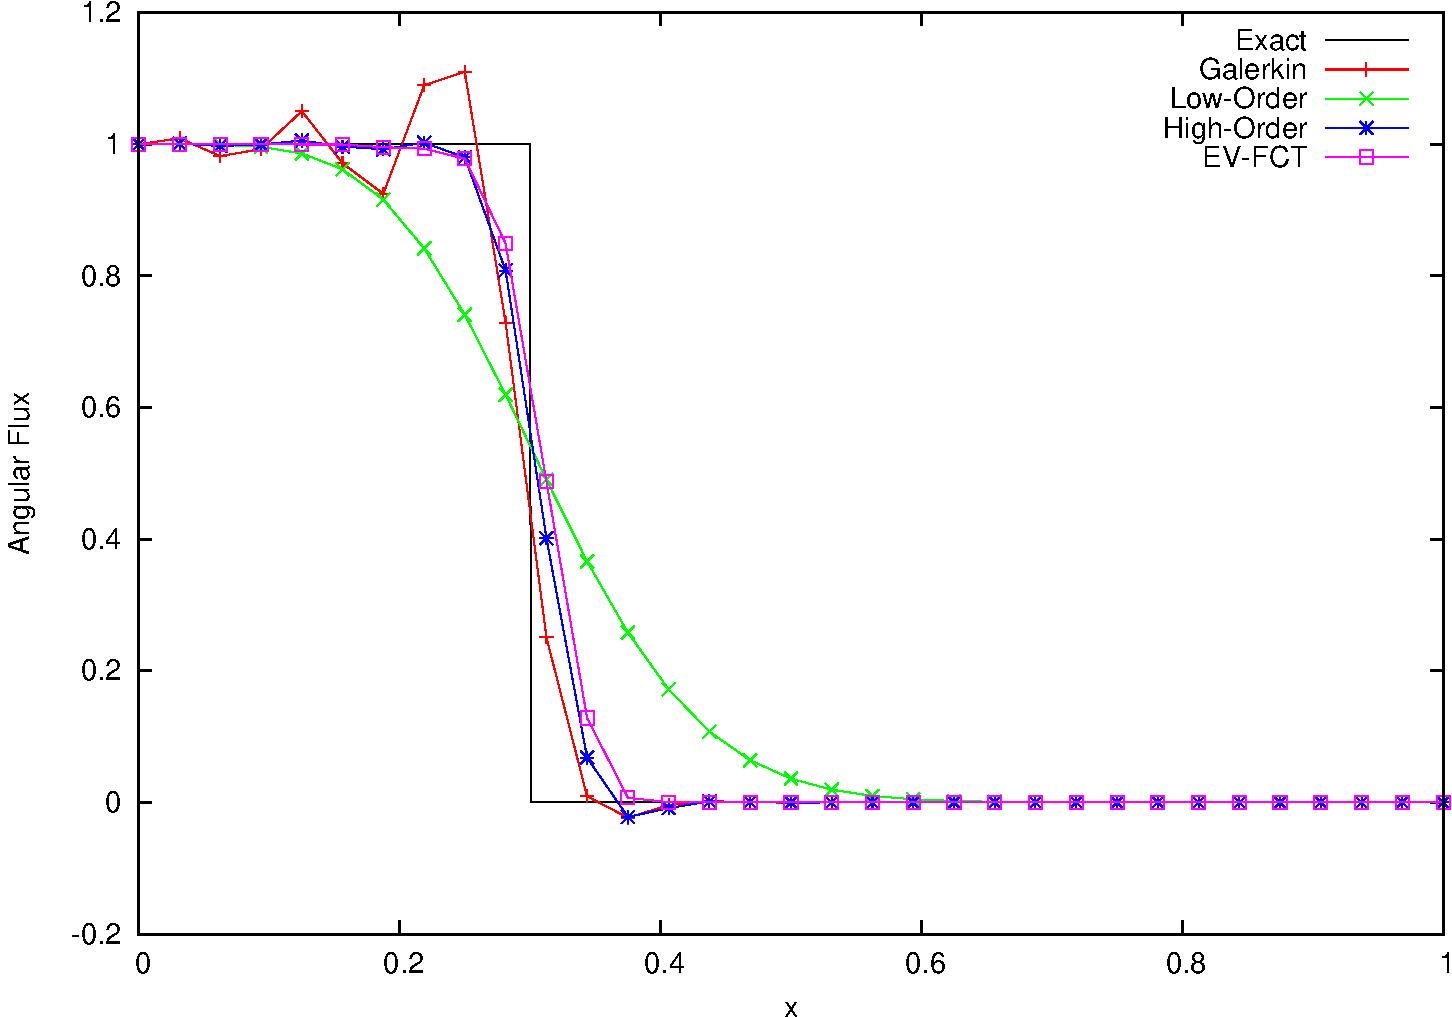
\includegraphics[width=0.20\textwidth]{figures/solutions_3_SSPRK33.pdf}

\bigskip

\underline{\bf Multidimensional test cases:} 

A $2 \times 2$ material layout (2D) and $2 \times 2 \times 2$ layout (3D)
where one material is a pure absorber and all other materials are void.


Radiation normally incident on one side (2D) or face (3D).
\medskip

\vspace{\baselineskip}

\begin{minipage}[t]{0.5\linewidth}
  \centering
  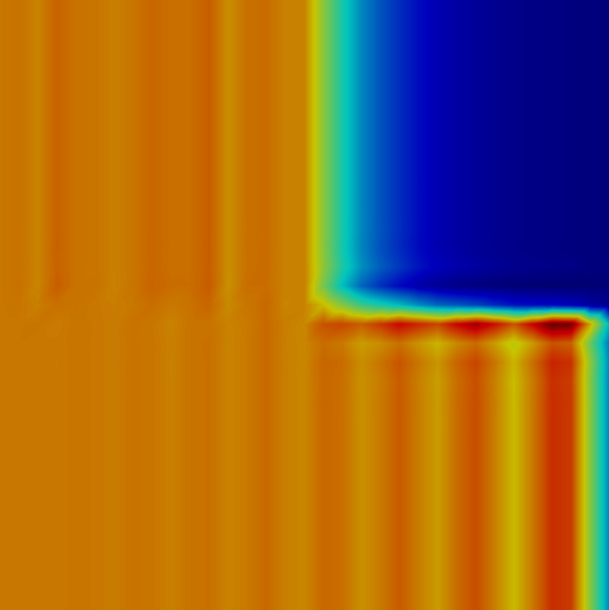
\includegraphics[width=\columnwidth]{figures/Gal2d.png}
  Galerkin
\end{minipage}
\begin{minipage}[t]{0.5\linewidth}
  \centering
  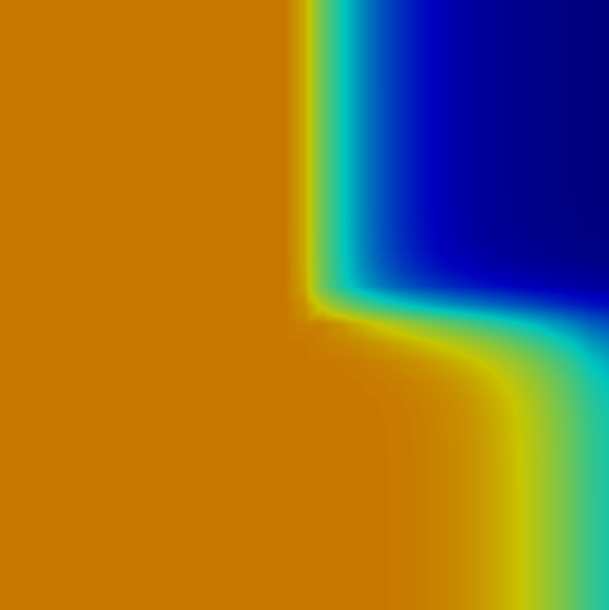
\includegraphics[width=\columnwidth]{figures/GalFCT2d.png}
  FCT
\end{minipage}

\begin{minipage}[t]{0.5\linewidth}
  \centering
  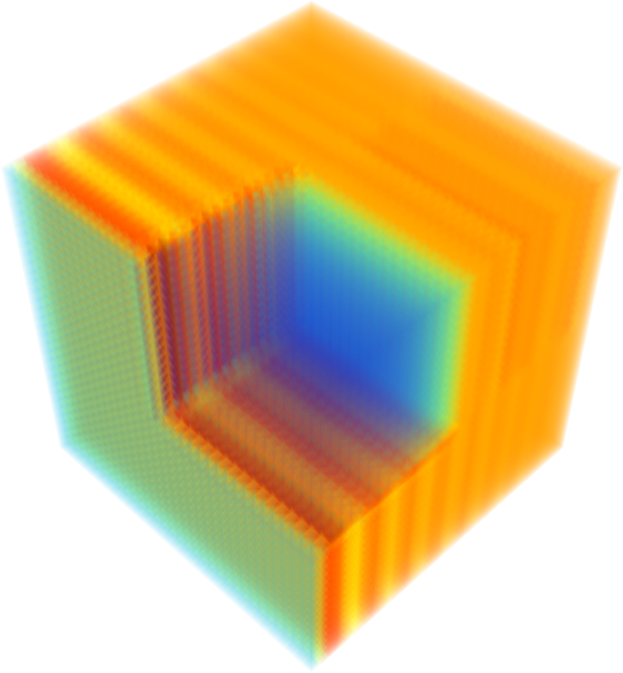
\includegraphics[width=\columnwidth]{figures/Gal_3D.png}
  Galerkin
\end{minipage}
\begin{minipage}[t]{0.5\linewidth}
  \centering
  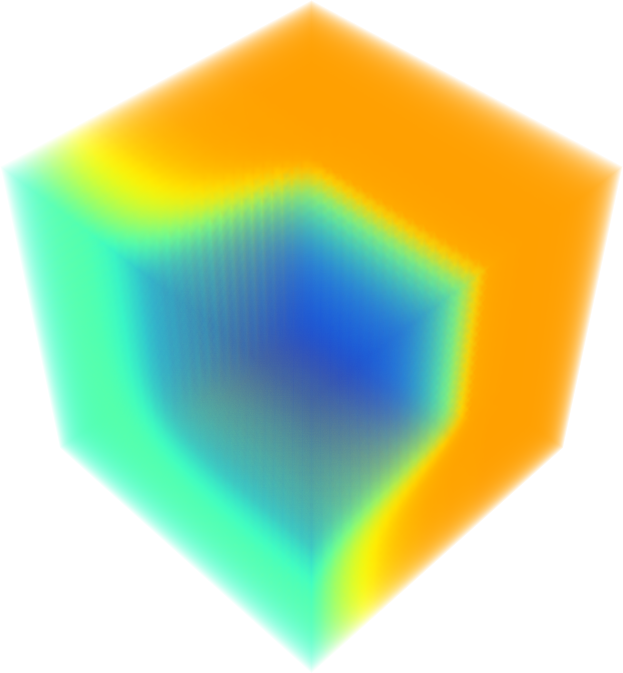
\includegraphics[width=\columnwidth]{figures/GalFCT_3D.png}
  FCT
\end{minipage}
